\documentclass{article}
\usepackage[utf8]{inputenc}
\title{Lecture 2 Gradient Descent, Stochastic Gradient Descent and Loss Functions}
\author{wbg231 }
\date{December 2022}
\newcommand{\R}{$\mathbb{R}$}
\newcommand{\B}{$\beta$}
\newcommand{\A}{$\alpha$}
\newcommand{\D}{\Delta}

\newcommand{\avector}[2]{(#1_2,\ldots,#1_{#2})}
\newcommand{\makedef}[2]{$\textbf{#1}$:#2 }
\usepackage{tikz,graphicx,hyperref,amsmath,amsfonts,amscd,amssymb,bm,cite,epsfig,epsf,url}

\begin{document}

\maketitle

\section{introduction}
\begin{itemize}
\item \href{https://nyu-ds1003.github.io/mlcourse/2023/lectures/lec02/02.pdf}{lecture slides}
\section{ERM review}
\subsection{unconstrained ERM}
\item ERM is empirical risk minimization 
\item the are three spaces 
\begin{itemize}
    \item the input space $X$
    \item the output space $Y$
    \item the action space $A$
\end{itemize}
\item the prediction function get an input $x\in X$ and produces an action $a\in A$ $$f:X\rightarrow A $$ $$\newline \quad x\rightarrow f(x)$$
\item the loss function evaluates an action in context of the outcome y $$\ell:A\times Y\rightarrow \mathbb{R}$$\\ $$\quad (a,y)\rightarrow \ell(a,y)$$
\item the risk of a prediction function $f:X\rightarrow A$ is $$R(f)=E[\ell(f(x),y)]$$
\item the Bayes prediction function $f^*:X\rightarrow A$ is a function that ac hives the minimal risk among all possible functions $$f^{*}\in argmin_{f}R(f)$$
\item the risk of the Bayes prediction function is called the Bayes risk 
\item let a dataset $D_{n}=((x_1,y_1)...(x_n,y_n))$ be iid with probability distribution $P_{X\times Y}$
\imte the empirical risk of $f:X\rightarrow A$ with respect to $d_n$ is $$\hat{R}_{n}=\frac{1}{n}\Sigma_{i=1}^{n}\ell(f(x_i),y_i)$$
\subsection{constrained ERM}
\item a hypothesis space $\mathcal{F}$ is a set of functions mapping $X\rightarrow A$ 
\item this is the set of predictions functions we are choosing from 
\item an empirical risk minimizer in $\mathcal{F}$ is $$\hat{f}_{n}\in argmin_{f\in\mathcal{F}}\frac{1}{n}\Sigma_{i=1}^{n}\ell(f(x_i),y_i)$$
\subsection{example: linear least squared regression}
\item input space $x\in \mathbb{R}^d$
\item output space $y\in \mathbb{R}$
\item action space $y\in \mathbb{R}$
\item loss function $\ell(\hat{y},y)=(y-\hat{y})^2$
\item hypothesis space $\mathcal{F}=\{f:\mathbb{R}^{d}\rightarrow \mathbb{R}| f(x)=w^{t}x,w\in \mathbb{R}^{d}\}$ that is linear functions mapping from $\mathbb{R}^{d}\rightarrow \mathbb{R}$
\imte our goal is to find the ERM $\hat{f}\in \mathcal{F}$
\item our empirical risk can be written as $\hat{R}_{n}=\frac{1}{n}\Sigma_{i=1}^{n}\ell(f(x_i),y_i)=\frac{1}{n}\_{i=1}^{n}(w^tx_i-y_i)^2$
\item we can solve this specific problem analytically with calculus but in general there is not an analytical way to get a solution. 
\section{gradient descent }
\item we assume that the objective function $f:\mathbb{R}^{d}\rightarrow \mathbb{R}$ is differentiable 
\item our goal is to find $x^{*}=argmin_{x\in \mathbb{R}^{d}}f(x)$ ie we want to find the  minimum arguments  of our objective. 
\item the gradient of f at point $x_0$ written as $\nabla_{x}f(x_0)$ is the direction which f(x) increases fastest if we start from $x_0$
\item 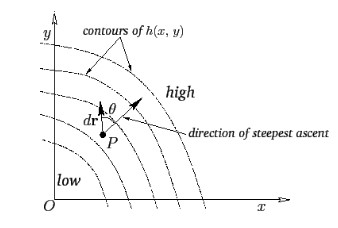
\includegraphics[width=5cm]{lecture_notes/lecture_2/immages/g_d_1.jpg}
\item so note here the gradient is perpendicular to the contour lines, this makes sense as the contour lines are the direction that keep our function value the same/
\item  to reach  minimum as quickly as possible we want to go in the opposite direction of the gradient
\item gd algorithm
\begin{itemize}
    \item initialize x
    \item repeat
    \begin{itemize}
        \item $x\rightarrow x-\alpha \nabla f(x)$
    \end{itemize}
    \item until the stopping criteria is satisfied 
\end{itemize}
\item the step size $\alpha\in \mathbb{R}$ is the amount which we update x each iteration. 
\item 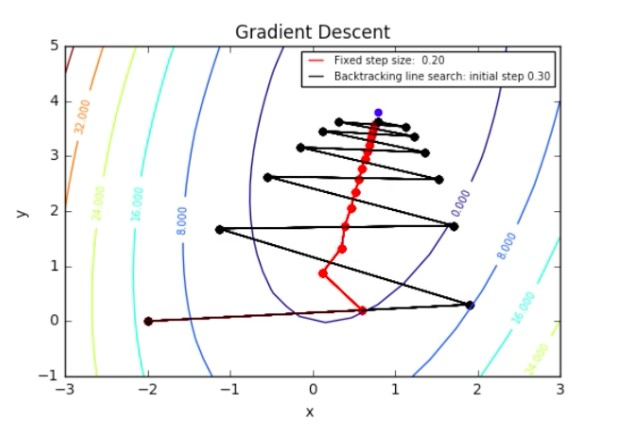
\includegraphics[width=5cm]{lecture_notes/lecture_2/immages/g_d_2.jpg} 
\item this is how to visualize gradient descent
\subsection{step size}
\item a fixed step size $\alpha$ will work eventually as long as it is small enough 
\begin{itemize}
    \item if $\alpha$ is to large the optimization may not converge
    \item in practice we often try a few values before going with one 
\end{itemize}
\subsection{convergence theorem}
\item suppose $f:\mathbb{R}^{d}\mathbb{R}$ is convex and differentiable and $\nabla f$ is Lipschitz continuous with constant $L>0$ ie $$||\nabla f(x)-\nabla f(x')||\leq L||x-x'||$$
$\forall x,x'\in \mathbb{r}^d$ then the gradient with fixed step size $\alpha \leq \frac{1}{L}$ converges in particular $$f(x_{k})-f(x^{*})\leq \frac{||x_{0}-x^{*}||^2}{2\alpha k}$$
\item Lipschitz continuous just means that the function in this case the gradient has a bounded rate of change (ie it does not jump really)
\item and this theorem tells us that given the function is convex, and differentiable and its gradient is Lipschitz continuous we Can bound how long it will take for gradient descent to converge.
\item further this tells us that if the conditions are met our gradient descent is grunted to converge in $O(\frac{1}{k})$
\subsection{ when to stop}
\item two broad choices of when to stop 
\item either pick some small $\epsilon \in \mathbb{R}$ and wait until $||\nabla f(x)||_{2}\leq \epsilon$ ie wait until our gradient is sufficiently close to zero (ie pretty close to a local min)
\item or early stopping ie evaluate the loss function after each iteration and stop when the loss does not improve or gets worse
\subsection{scaling issues}
\item recall that we run the gradient descent on the empirical loss function $$\hat{R}_{n}(2)=\frac{1}{n}\Sigma_{i=1}^{n}\ell(f_{w}(x_i),y_i)$$
\item however in gradient descent we need to convert the gradient of our function at each iteration meaning we compute the gradient $\nabla \hat{R}_{n}(w)=\frac{1}{n}\Sigma_{i=1}^{n}\nabla_{W}\ell(f_{w}(x_i),y_i)$
\item thus we need to go over all training points in each iteration meaning our algorithm will scale in $O(n)$ time which is not efficient over really large data sets. 
\section{stochastic gradient descent}
\item stochastic just means randomly determined .
\item so instead of using the gradient we use some estimate of the gradient 
\item this can work well
\item intuition 
\begin{itemize}
    \item gradient descent is iterative anyway 
    \item so at every step we have a chance to recover from errors that we make in estimation 
\end{itemize}
\item the full gradient is $\nabla \hat{R}_{n}(w)=\frac{1}{n}\Sigma_{i=1}^{n}\nabla_{W}\ell(f_{w}(x_i),y_i)$ this is the average over the full batch of our dataset $D_{n}=((x_1,y_1),...(x_n,y_n))$
\item we can call a mini batch a random sub sample of our data of size k $((x_{m1},y_{m1}),...(x_{mk}, y_{mk})$
\item thus we can define a mini batch gradient as $\nabla\hat{R}_{k}-\frac{1}{k}\Sigma_{i=1}^{k}\nabla w \ell(f_{w}(x_{mi}, y_{mi})$ in other words we are just taking the gradient over the mini batch ie a random sub bag of our data.
\item stochastic gradient descent is minibatch gradient descent with mini batch size =1 that is $\nabla\hat{R}_{1}-\nabla w \ell(f_{w}(x_{m}, y_{m})$
\item rule of thumb for stochastic methods 
\begin{itemize}
    \item they work well far from the optimum, ie they get the general trend of gradient 
    \item but struggle close to the optimum this is where the noise of sampling can be tough 
\end{itemize}
\subsection{mini batch gradient properties}
\item the mini batch gradient is an unbiased estimator of the full batch gradient ie $$E[\nabla \hat{R}_{k}(w)]=\nabla \hat{R}_{n}(w)$$ this more or less means in the expectation or on average our mini batch will get the gradient correct.
\item the bigger the mini batch the better the estimate. $$\frac{1}{k}var(\nabla \hat{R}_{1}(w))=var[\nabla \hat{R}_{k}(w)]$$ 
\item this is more or less saying that the gradient of  a mini batch of size k will have $\frac{1}{k}$ times the variance of the gradient of a mini batch of size 1. 
\item trade off of mini batch size
\begin{itemize}
    \item bigger k $\Rightarrow$ better estimate of the gradient but slower
    \item smaller k $\Rightarrow$ worse estimate of the gradient but fast. 
\end{itemize}
\subsection{convergence of Stochastic Gradient Descent }
\item to grantee convergence we want to use a diminishing step size for example $\alpha_{k}=\frac{1}{k}$
\item Theoretically GD is much faster than SGD in terms of convergence 
\begin{itemize}
    \item but that is mostly because SGD does not close in on the exact min very which , but in many real cases we don't care that much about optimization to a high accuracy. 
\end{itemize}
\item mini batch gradient descent algorithm 
\begin{itemize}
    \item initialize w
    \item repeat until stopping condition
    \begin{itemize}
        \item randomly chose a bag of size k from our data set ie $\{(x_i,y_i\}_{i=1}^{k}\subset D_n$ 
        \item update our weights $W\rightarrow - \alpha [\frac{1}{n}\Sigma_{i=1}^{n}\nabla_{w}\ell(f_{w}(x_i),y_i)]$
    \end{itemize}
\end{itemize}
\subsection{logistic reg with l2 norm }
\item 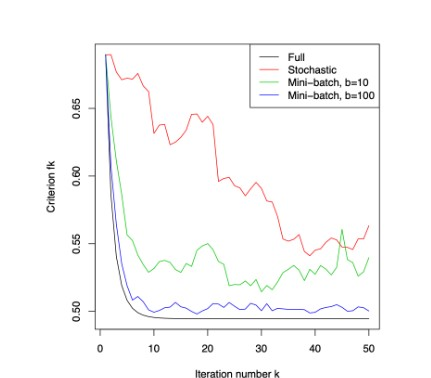
\includegraphics[width=5cm]{lecture_notes/lecture_2/immages/g_d_3.jpg}
\item full batch methods converge faster 
\item 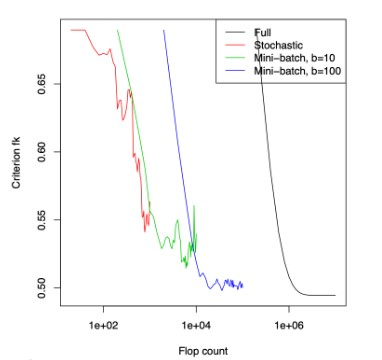
\includegraphics[width=5cm]{lecture_notes/lecture_2/immages/g_d_4.jpg}
\item mini batch methods are more computationally efficient
\item 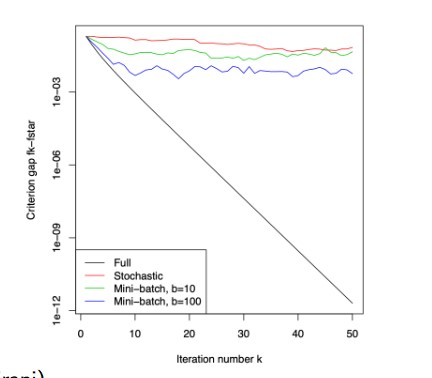
\includegraphics[width=5cm]{lecture_notes/lecture_2/immages/g_d_5.jpg}
\item batch methods are faster closer to the optimum 



\section{loss functions: regression}
\subsection{problem set up}
    \item input space $X=\mathbb{R}^{d}$
    \item action  space $A=\mathbb{R}$
    \item output space $y=\mathbb{R}$
    \item $\hat{y}$ is our predicted outcome, $y$ is our observed outcome 
\subsection{loss function properties}
\item a loss function in general maps $$(\hat{y},y)\rightarrow \ell(\hat{y},y)\in \mathbb{R}$$
\item most regression loss functions only depend on the residual ie $r=y-\hat{y}$ which is how far our prediction was from the true outcome, or what you have to add to your prediction to get the true outcome
\item a loss function $\ell(\hat{y},y)$ is called distance based if 
\begin{itemize}
    \item it only depends on the residual $$\ell(\hat{y},y)=\psi(y-\hat{y}$$ for some $\psi: \mathbb{R}\rightarrow \mathbb{R}$
    \item it is zero residual when $$\psi(0)=0$$
\end{itemize}
\item distance based loss functions are transition invariant so that is $\ell(\hat{y}+b,y+b)=\ell(\hat{y},y)\forall b\in \mathbb{R}$
\item sometimes we use the natural error $\frac{\hat{y}-y}{y}$
\item usually we can transform the loss to be translation invariant 
\subsection{example loss functions}
\item call the residual $r=\hat{y}-y$
\item square or $\ell_{2}$ loss is $\ell(r)=r^2$
\item absolute $\ell_{1}$ or Laplace loss is $\ell(r)=|r|$
\item robustness is how much a loss function is effected by outliers 
\item absolute loss is robust to outliers, squared loss is not robust
\item also not that square loss is differentiable while absolute loss is non differentiable 
\item Huber loss is quadratic for $|r|\leq  \delta$ and linear for $|r|> \delta$ this allows it to be both robust to outliers and differentiable everywhere. 
\item graphs of regression loss functions\\
 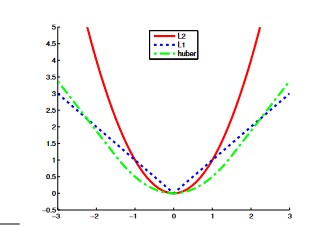
\includegraphics[width=5cm]{lecture_notes/lecture_2/immages/g_d_6.jpg}
 \subsection{classification loss functions }
\subsection{classification problem}
\item input space $X\in \mathbb{R}^{d}$
\item outcome space $y\in \{-1,1\}$ (for binary classification)
\item action space $A=\mathbb{R}$ this is easier to work with than just $\{-1,1\}$
\item then we make a prediction $a=f(x)>0\rightarrow $ predict 1 
\item $a=f(x)<0\rightarrow $ predict 0
\item $|f(x)|$ reflects our confidence in the estimate ie high values mean our function is very confident 
\subsection{score function}
\item our prediction function  $f:X\rightarrow \mathbb{R}$
\item the value $f(X)$ is called the score of the input x. 
\item f may be called teh score function 
\item $|f(x)|$ reflects our confidence in the estimate ie high values mean our function is very confident
\subsection{margin}
\item a margin or functional margin for a predicted score $\hat{y}$ and the true class $y\in \{-1,1\}$ is $$y\hat{y}=yf(x)$$
\item the margin is a measure of how correct we are 
\begin{itemize}
    \item if y and f(x) have the same sign the prediction is correct and the margin is positive
    \item is y and f(x) have opposite signs prediction is incorrect and the margin is negative
\end{itemize}
\item we want to max the margin of our estimation
\item most classification loss functions depend on the margin ie they are margin based loss functions. 
\subsection{some classification loss functions}
\item let $\Tilde{f}$ be the inference function mapping $\Tilde{f}(f(x))=1$ if $f(x)>0$ and $\Tilde{f}(f(x))=-1$ if $f(x)<0$
\item the 0-1 loss function $f:X\rightarrow\{-1,1\}$ is $$\ell(f(X),y)=1(f(x)\neq y)$$ so that is the loss is zero if the prediction is correct and 1 if the prediction is incorrect.
\item the empirical risk for the 0-1 loss is $$\hat{R}_{n}(f)=\frac{1}{n}\Sigma_{i=1}^{n}1(y_if(x_i)\leq 0)$$
\item note that empirical risk for 0-1 loss is neither convex nor differentiable so it is hard to optimize
\item hinge loss $$\ell_{hinge}=max(1-m,0)$$ hinge loss is convex but not differentiable at m=1
\item logistic or log loss is $$\ell_{logistic}=log(1+e^{-m})$$
\item recall that in regression squared loss was $\ell(f(x),y)=(f(x)-y)^2$
\item we can write squared loss for classification in terms of the margin m $$\ell(f(x),y)=(f(x)-y)^2=(f(X)^2-2f(x)y+y^2)=(1-f(x)y)^2=(1-m)^2$$ since $y^2=1$
\item square loss is convex and differentiable everywhere but not robust to outliers.
\item graph of classification loss functions \\ 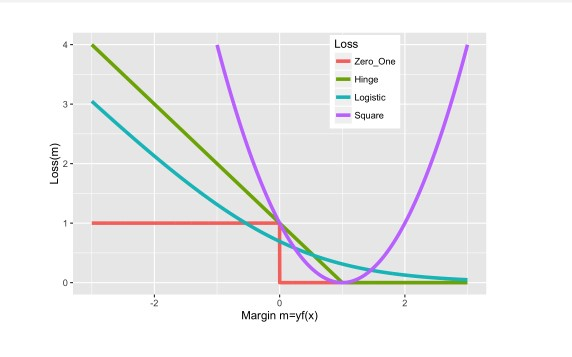
\includegraphics[width=7.5cm]{lecture_notes/lecture_2/immages/g_d_7.jpg}
\end{itemize}
\end{document}
